% !TeX spellcheck = pt_PT
\chapter{Sistema de Odometria Visual} \label{chap:sist}

Neste capítulo serão apresentados os procedimentos implementados para a realização dos testes. O capítulo aborda o \textit{software} e \textit{hardware} utilizados no desenvolvimento.

\section{Software}

Neste subcapítulo serão descritas as ferramentas de \textit{software} utilizadas assim como o código produzido.

\subsection{ROS}

ROS (\textit{Robot Operating System}) é uma \textit{framework} para desenvolvimento de \textit{software} de robótica. ROS consiste num compêndio de bibliotecas, ferramentas e outros recursos que visa facilitar a criação de comportamentos complexos alcançando uma vasta gama de plataformas robóticas distintas. 

O ROS fornece serviços idêntico a um sistema operativo, incluindo abstração de \textit{hardware}, baixo nível de controlo, implementação de funcionalidades e mensagens que são transmitidas entre nós. Além disto, é constituído por bibliotecas e ferramentas para obter, criar, gravar e executar código em vários computadores. 

Desta forma, ROS é caracterizado por:

\begin{itemize}
	\item \textbf{Pacotes} - O \textit{software} desenvolvido em ROS organiza-se em pacotes. Os pacotes são módulos que podem conter nós, bibliotecas independentes, \textit{datasets}, ficheiros de configuração, elementos de \textit{softwares} de terceiros, entre outros elementos que constituem o módulo. Os pacotes constituem a unidade base de compilação.
	\item \textbf{Nós} - Os nós são processos em ROS que executam computação, funcionando como programas. Os nós comunicam entre si através da publicação e subscrição de mensagens, serviços e através do \textit{Parameter Server}. Um sistema robótico em execução utiliza um conjunto de nós que cooperam para o seu funcionamento. A arquitetura distribuída de ROS permite que os nós em execução não necessitem de operar no mesmo equipamento, possibilitando a simbiose de diferentes plataformas comunicando entre si. O nó mestre pertence ao conjunto de nós laçando pelo \textit{roscore}, e tem a função de possibilitar aos nós que se localizem uns aos outros permitindo o estabelecimento de comunicações. 
	\item \textbf{Tópicos} - Os tópicos são os recipientes através dos quais os nós trocam mensagens entre si. Os tópicos utilizam um modelo de publicação/subscrição que separa a produção de informação do seu consumo. Os nós não têm conhecimento de outros nós que publiquem determinado tópico ou o subscrevam. Um nó apenas necessita de subscrever os dados específicos a um tópico ou de publicar dados num tópico específico. A estrutura permite a existência de múltiplos publicadores e subscritores associados a cada tópico.
	\item \textbf{Serviços} - A unidirecionalidade existente no modelo publicador/subscritor não possibilita interações do tipo "pedido/resposta". Para possibilitar este tipo de interações existem os serviços em ROS. Um serviço é composto por um par de mensagens, uma mensagem definida para o pedido e outra para a resposta. Um nó pode oferecer um serviço ativado por um nó cliente ao submeter a mensagem de pedido.
	
\end{itemize}

A biblioteca de ROS suporta o desenvolvimento ROS em linguagem C++ e Python.


\subsubsection{Nó VisodoAgro}

O algoritmo implementado neste nó pode ser resumido no diagrama de ação ~\ref{fig:diaguml}

\begin{figure}[h!] %colocar figura a seguir ao texto anterior
	\begin{center}
		\leavevmode		
		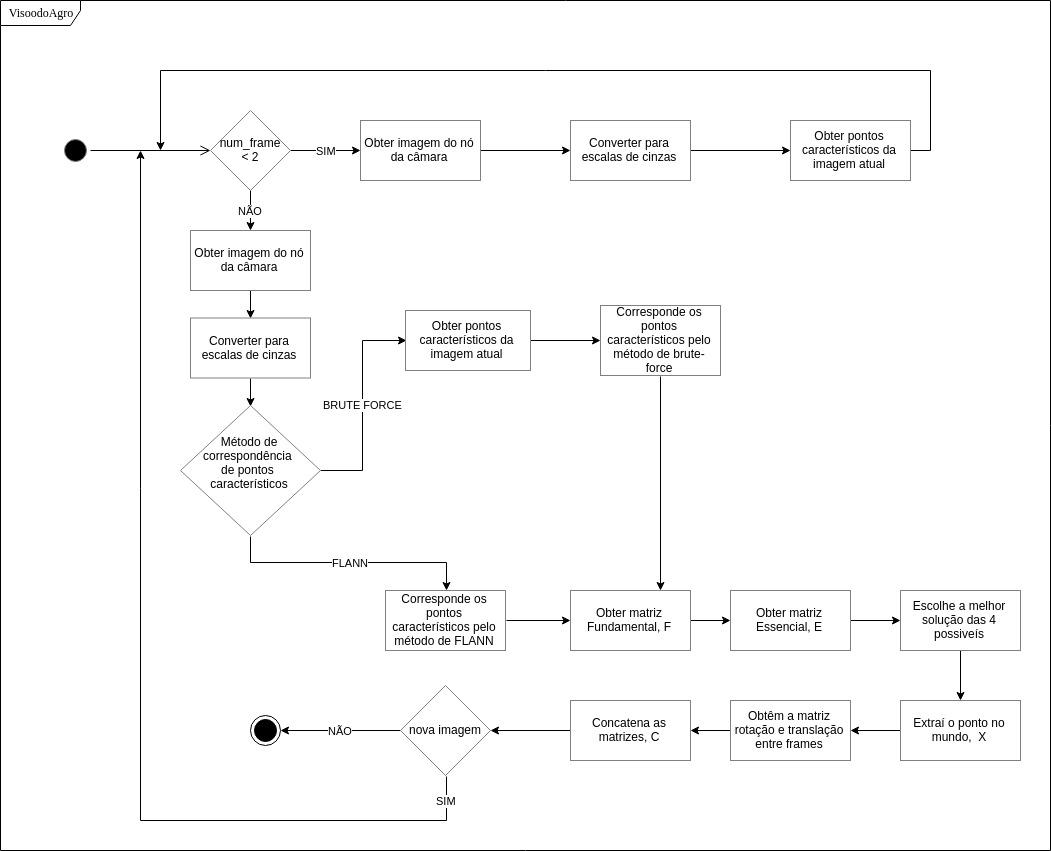
\includegraphics[width=1\textwidth]{umldiagram.jpg}
		\caption{Diagrama de ação do nó implementado em ROS.}
		\label{fig:diaguml}
	\end{center}
\end{figure}



No primeiro frame o algoritmo lê a imagem e transforma em escala de cinzas. De seguida, calcula os pontos característicos da imagem. Visto que no primeiro frame não é possível realizar uma correspondência com o frame anterior, devido à inexistência deste, o algoritmo avança para o próximo frame. A partir do segundo frame os passos são sempre iguais. Assim, o algoritmo obtêm o próximo frame e extraí a imagem em escala de cinzas . Seguidamente. caso se utilize o método de \textbf{brute force} , explicito no capitulo ~\ref{subchap:BRUTE}, calcula-se os pontos característicos deste frame que corresponderam aos pontos característicos do anterior. Caso o método seja \textbf{FLANN}, explicito no capitulo ~\ref{subchap:FLANN}, utiliza-se uma pequena região à volta dos pontos característicos do frame anterior como forma de se encontrar o ponto característico do frame atual. 


Obtida a matriz com as devidas correspondências é necessário calcular a matriz Fundamental. Esta, é obtida através de um loop em que escolhe um conjunto de correspondências aleatoriamente de forma a calcular a matriz fundamental. De seguida testa a qualidade dessa matriz Fundamental através do numero de inliers \footnote{pontos onde está a maior concentração de pontos.}, guardando o conjunto de correspondências com maior número de inliers. No fim calcula a matriz Fundamental com o melhor conjunto de correspondência.

%\textbf{Expressar como a matriz fundamental é calculada.}

\begin{figure}[h!] %colocar figura a seguir ao texto anterior
	\begin{center}
		\leavevmode		
		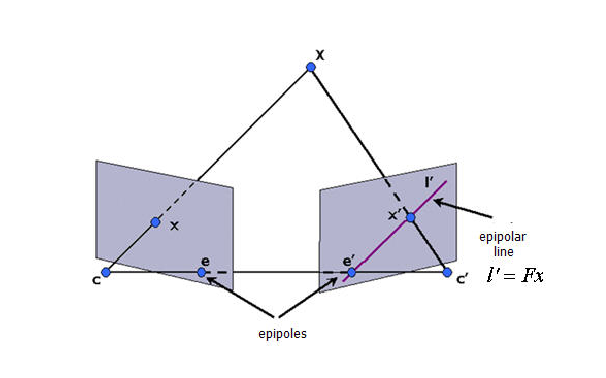
\includegraphics[width=0.6\textwidth]{epipolar.png}
		\caption{Representação da linha epipolar.}
		\label{fig:equ}
	\end{center}
\end{figure}

Como representado na figura ~\ref{fig:equ} o ponto \textbf{x} corresponde ao ponto no plano de imagem do frame anterior, \textbf{x'} corresponde ao ponto no plano de imagem do frame atual que corresponde os dois ao ponto \textbf{X} no mundo. Desta forma, \textbf{Fx} descreve uma linha (linha epipolar) na qual o ponto correspondente \textbf{x'} na outra imagem deve estar. Isto significa que, para todos os pares de pontos correspondentes: \[ {x}'^{T} F x = 0 \] 
sendo, \[ F =  \left[ \begin{array}{ccc}
f_{11} & f_{12} & f_{13} \\ 
f_{21} & f_{22} & f_{23} \\ 
f_{31} & f_{32} & f_{33} 
\end{array}\right], \] \[ {x}' = \left[ \begin{array}{ccc}
{u}' \\ {v}'\\ 1 
\end{array} \right] e  \thinspace x = \left[ \begin{array}{ccc}
u \\ v \\ 1  \end{array}\right]  . \]

Desenvolvendo, obtemos : \[ u'uf_{11} + u'vf_{12} + u'f_{13} + v'uf_{21} + v'vf_{22} + v'f_{23} + uf_{31} + vf_{32} + f_{33} = 0 \]

\[	\Leftrightarrow (u'u , u'v , u' , v'u , v'v , v' , u , v , 1) \left( \begin{array}{ccccccccc}
f_{11}\\
f_{12}\\
f_{13}\\
f_{21}\\
f_{22}\\
f_{23}\\
f_{31}\\
f_{32}\\
f_{33}
\end{array} \right) = 0 \] 

Para todos os pontos característicos : \[  \left[ \begin{array}{ccccccccc }
u'_{1}u_{1} & u'_{1}v_{1} & u'_{1} & v'_{1}u_{1} & v'_{1}v_{1} & v'_{1} & u_{1} & v_{1} & 1 \\ 
\vdots  & \vdots  & \vdots  & \vdots  & \vdots  & \vdots  & \vdots  & \vdots  & \vdots \\ 
u'_nu_n & u'_nv_n & u'_n & v'_nu_n & v'_nv_n & v'_n & u_n & v_n & 1
\end{array}\right] \left( \begin{array}{ccccccccc}
f_{11}\\
f_{12}\\
f_{13}\\
f_{21}\\
f_{22}\\
f_{23}\\
f_{31}\\
f_{32}\\
f_{33}
\end{array} \right) = 0 \]  \begin{equation}\label{equ:af=0}
\Leftrightarrow \textbf{AF = 0}. 
\end{equation}

Sendo a matriz \textbf{A} invertível, singular  e o número de pontos característicos superior a 8, a solução é obtida através da decomposição em valores singulares (SVD, do inglês \textit{singular value decomposition}).  \[ F = U D V^{T}.\]

%\textbf{Expressar como é obtida a matriz Essencial através da decomposição de valores singulares}

Conseguida a matriz Fundamental e conhecida a matriz de parâmetros Intrínsecos , \textbf{K}, a matriz Essencial, que representa o plano epipolar na imagem ~\ref{fig:esseciallinemat}, é obtida pela seguinte equação:
\[ E = {K}'^{T} F K, \]  sendo \[ E = R \left[\begin{array}{c}
t
\end{array}\right]_{x} \], onde \textbf{R} é a matriz rotação e \textbf{t} é a matriz translação.

\begin{figure}[h!] %colocar figura a seguir ao texto anterior
	\begin{center}
		\leavevmode		
		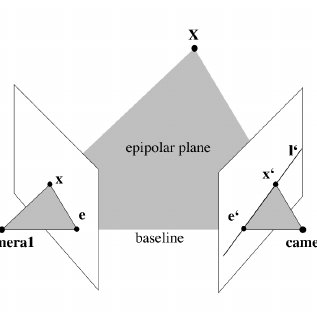
\includegraphics[width=0.6\textwidth]{epipolar2.jpg}
		\caption{Representação do plano epipolar.}
		\label{fig:esseciallinemat}
	\end{center}
\end{figure}

Sendo a matriz Essencial descrita desta forma, é possível obter os valores das matrizes rotação e translação através da decomposição dos valores singulares (\textbf{SVD}). Sendo : \[ E = U diag(1,1,0) V^{T} \] onde as duas soluções possíveis para a matriz rotação, R: \[ R = UWV^T \] \[ R = UW^TV^T \] e a matriz translação, t: \[ t = \pm u_3 \].


Obtidas as matrizes rotação e translação existem 4 possíveis soluções, tal como verificado anteriormente. Desta forma, é necessário escolher a solução certa. Para testar as hipóteses é realizada a triangulação por regressão ortogonal e escolhida a solução mais consistente.

Assim, é possivel verificar que exite uma relação entre os pontos correspondentes entre imagens. Se um ponto desconhecido no mundo, \textbf{X}, representado na frame anterior como \textbf{x} e no frame atual como \textbf{x'}, as coordenadas de \textbf{X} podem ser calculadas. Isto, requer a matriz Intrínseca e a matriz Essencial entre frames.

A relação entre os pontos da imagem, \textbf{x} e \textbf{x'} e o ponto no mundo \textbf{X} com os parâmetros da câmara P é expressa \[ x = P X \] \[ x' = P'X \], onde P e P' $\epsilon$  $\mathbb{R}^{3x4}$ é a combinação da matriz Intrínseca e Essencial do frame anterior e atual, respetivamente.

Sendo, \[ x =  \left[ \begin{array}{ccc} u \\ v \\ 1 \end{array} \right],  x' =  \left[ \begin{array}{ccc} u' \\ v' \\ 1 \end{array} \right] ,  X =  \left[ \begin{array}{cccc} X_w \\ Y_w \\ Z_w \\ 1 \end{array} \right] \], \[ E =  \left[ \begin{array}{cccc} r_{11} & r_{12} & r_{13} & t_{x} \\ r_{21} & r_{22} & r_{23} & t_{y} \\ r_{31} & r_{32} & r_{33} & t_{z} \\ \end{array} \right] , K =  \left[ \begin{array}{ccc} f_x & 0 & x_c \\ 0 & f_y & y_c \\ 0 & 0 & 1 \\ \end{array} \right] \].

E considerando $p^{iT}$ as linhas da matriz P e devido à estrutura da matriz Intrínseca, K, X é expresso pela seguinte equação linear :  \begin{equation}\label{equ:svdMatcs} 
\left[ \begin{array}{cccc}
up^{3T} - p^{1T} \\
vp^{3T} - p^{2T} \\
u'p'^{3T} - p'^{1T} \\
v'p'^{3T} - p'^{2T} 
\end{array} \right] X = 0 .
\end{equation}

A equação ~\ref{equ:svdMatcs} é resolvida através da decomposição em valores singulares como explicito anteriormente na equação ~\ref{equ:af=0}.

Desta forma, \[ X = UDV^T. \] 

Onde, X $\epsilon$ $\mathbb{R}^{1xn}$ e n igual ao número de pontos característicos com correspondência.
Através da matriz X é obtida a matriz Rotação e Translação resultante da transformação .

\begin{figure}[h!] %colocar figura a seguir ao texto anterior
	\begin{center}
		\leavevmode		
		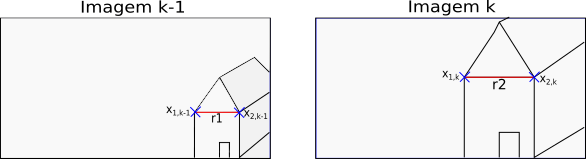
\includegraphics[width=0.6\textwidth]{ration.png}
		\caption{Representação da razão entre frames.}
		\label{fig:ration}
	\end{center}
\end{figure}

Como ilustado na figura ~\ref{fig:ration} a escala entre frames é obtida pela razão, r, entre a distância de dois pontos em frames difrentes. Considerando \textit{$x_{1,k-1}$} , \textit{$x_{2,k-1}$} ,\textit{$x_{1,k}$} ,\textit{$x_{2,k}$} pontos na imagem com coordenadas (u,v) resulta : \[ r = \frac{\left \| x_{1,k-1} - x_{2,k-1} \right \|}{\left \| x_{1,k} - x_{2,k} \right \|} \] .

\begin{figure}[h!] %colocar figura a seguir ao texto anterior
	\begin{center}
		\leavevmode		
		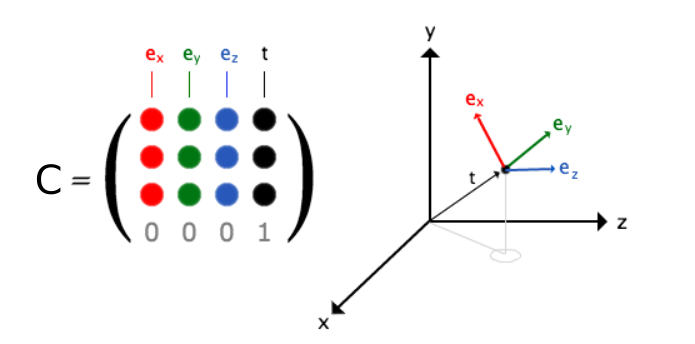
\includegraphics[width=0.6\textwidth]{homog.png}
		\caption{Representação da transformação homogénea.}
		\label{fig:homog}
	\end{center}
\end{figure}

\vspace{5mm}  %espaço de 5mm para figura ficar antes do seguinte texto

Desta forma, considerando a matriz rotação entre frames \[  R_f = \left[ \begin{array}{cccc}
r_{11} & r_{11} & r_{11} & t_1 \\ 
r_{21} & r_{22} & r_{23} & t_2 \\ 
r_{31} & r_{32} & r_{33} & t_3 
\end{array} \right] = \left(\begin{array}{ccc}
r_1 \\ r_2 \\ r_3
\end{array}\right)\]

e a matriz translação entre frames \[ t_f = \left[ \begin{array}{ccc}
t_x \\ t_y \\ t_z
\end{array}\right]\]

Onde , a matriz rotação global \[ R = R * R_f\]
e a matriz translação global \[ t = t + R * ( t_f * r ) . \]

Originando a matriz concatenação C, \[ C = \left[ R | t \right] = \left[ \begin{array}{cccc}
r_{11} & r_{11} & r_{11} & t_1 \\ 
r_{21} & r_{22} & r_{23} & t_2 \\ 
r_{31} & r_{32} & r_{33} & t_3 \\ 
0 & 0 & 0 & 1
\end{array} \right] \] 






Em termos de tópicos desenvolvidos no nó \textbf{visodoAgro}, foram criadas as seguintes mensagens customizadas : \textit{"msgInfo"}, \textit{"msgTime"} e \textit{"visodom"}, como representado na figura ~\ref{fig:rosgraph}

\begin{figure}[h!] %colocar figura a seguir ao texto anterior
	\begin{center}
		\leavevmode		
		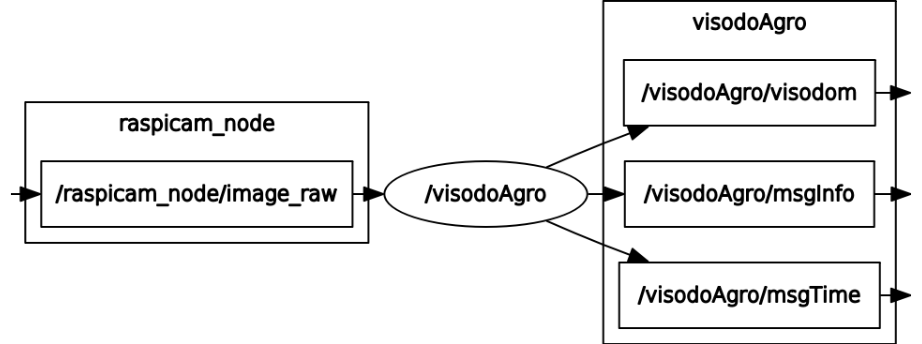
\includegraphics[width=1.5\textwidth]{rosgraph2.png}
		\caption{Representação dos tópicos elaborados no nó visodoAgro.}
		\label{fig:rosgraph}
	\end{center}
\end{figure}

Desta forma, o formato da mensagem \textbf{"msgInfo"} é representado pela figura  ~\ref{fig:msgInfo}

 \begin{figure}[h!] %colocar figura a seguir ao texto anterior
 	\begin{center}
 		\leavevmode		
 		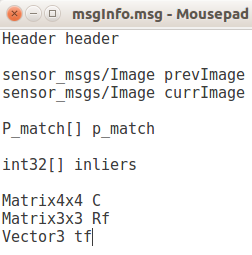
\includegraphics[width=0.4\textwidth]{msgInfo.png}
 		\caption{Conteúdo da mensagem \textit{msgInfo.msg}.}
 		\label{fig:msgInfo}
 	\end{center}
 \end{figure}
 



Esta mensagem é utilizada para publicar todos os dados importantes do algoritmo, para posteriormente ser realizada uma análise em Matlab e uma representação dos resultados obtidos nesta dissertação. 
Desta forma, nos campos \textbf{prevImage} e \textbf{currImage} são publicadas as imagens utilizadas para o cálculo das matrizes rotação e transformação nesse instante. Estas matrizes são publicadas no campos \textbf{Rf} e \textbf{tf}, respetivamente. 
O Campo \textbf{C} é usado para publicar a matriz concatenação, enquanto que o campo  \textbf{p\_match} é utilizado para publicar as correspondencias dos pontos caracteristicos. Além disso, existem ainda os \textit{inliers}, pontos utilizados para o cálculo das matrizes resultantes, removendo as correspondências que provocavam erros nos resultados.  


Por outro lado, a mensagem \textbf{"msgTime"} é utilizada para comparar os tempos de execução, o número imagens perdidas entre o processamento e quantidade de imagens processadas por diferentes tipos de algoritmos. Esta, é representada pelos seguintes campos da figura ~\ref{fig:msgTime}

\begin{figure}[h!] %colocar figura a seguir ao texto anterior
	\begin{center}
		\leavevmode		
		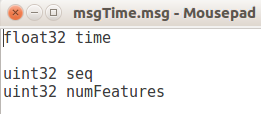
\includegraphics[width=0.4\textwidth]{msgTime.png}
		\caption{Conteúdo da mensagem \textit{msgTime.msg}.}
		\label{fig:msgTime}
	\end{center}
\end{figure}



Por fim, a mensagem \textbf{"visodom"} é utilizada para publicar a localização em relação ao primeiro frame. Esta, é constituída pelos seguintes parâmetros da figura ~\ref{fig:visodom}

\begin{figure}[h!] %colocar figura a seguir ao texto anterior
	\begin{center}
		\leavevmode		
		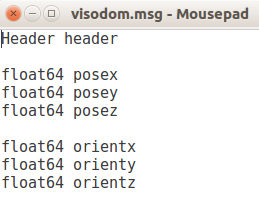
\includegraphics[width=0.4\textwidth]{visodom.png}
		\caption{Conteúdo da mensagem \textit{visodom.msg}.}
		\label{fig:visodom}
	\end{center}
\end{figure}

As coordenadas x, y e z são publicadas nos parâmetros \textbf{posex}, \textbf{posey}, \textbf{posez}, respetivamente e a orientação x,y e z nos parâmetros \textbf{orientx}, \textbf{orienty}, \textbf{orientz}, respetivamente. 





\subsection{Desenvolvimento em Matlab}

O Matlab é um \textit{software} de alto desempenho desenvolvido para o cálculo numérico. Caracteriza-se por implementar uma linguagem própriam, que resulta de uma combinação de linguagens como C, Java e Basic.

O código desenvolvido em Matlab teve como principal função o processamento dos dados guardados nos \textit{rosbags}. Estes \textit{rosbags} contêm as mensagens publicadas para cada teste realizado. Foram desenvolvidos \textit{scripts} para filtrar os dados de interesse e gerar dados possíveis de analisar e inferir conclusões.


\section{Hardware}

Este subcapítulo visa apresentar os componentes de hardware, utilizado no desenvolvimento do projeto.

\subsection{Raspberry Pi}

O Raspberry Pi é um computador do tamanho de um cartão de crédito, em que todo o hardware é integrado numa única placa. O principal objetivo é promover o ensino em Ciência da Computação básica em escolas, mas devido à sua excelente qualidade / preço é bastante usado em grandes projetos de robótica, programação e até aplicações industriais. 

O modelo utilizado nesta dissertação é o Raspberry Pi 3 model B. Este modelo contém um processador 1.2 GHz 64-bit quad-core ARMv8 CPU, 1 GB de RAM e Bluetooth 4.1. Além disto, este computador é compatível com ROS Kinetic e com vários módulos, como a câmara com lente olho de peixe.

\begin{figure}[h!] %colocar figura a seguir ao texto anterior
	\begin{center}
		\leavevmode		
		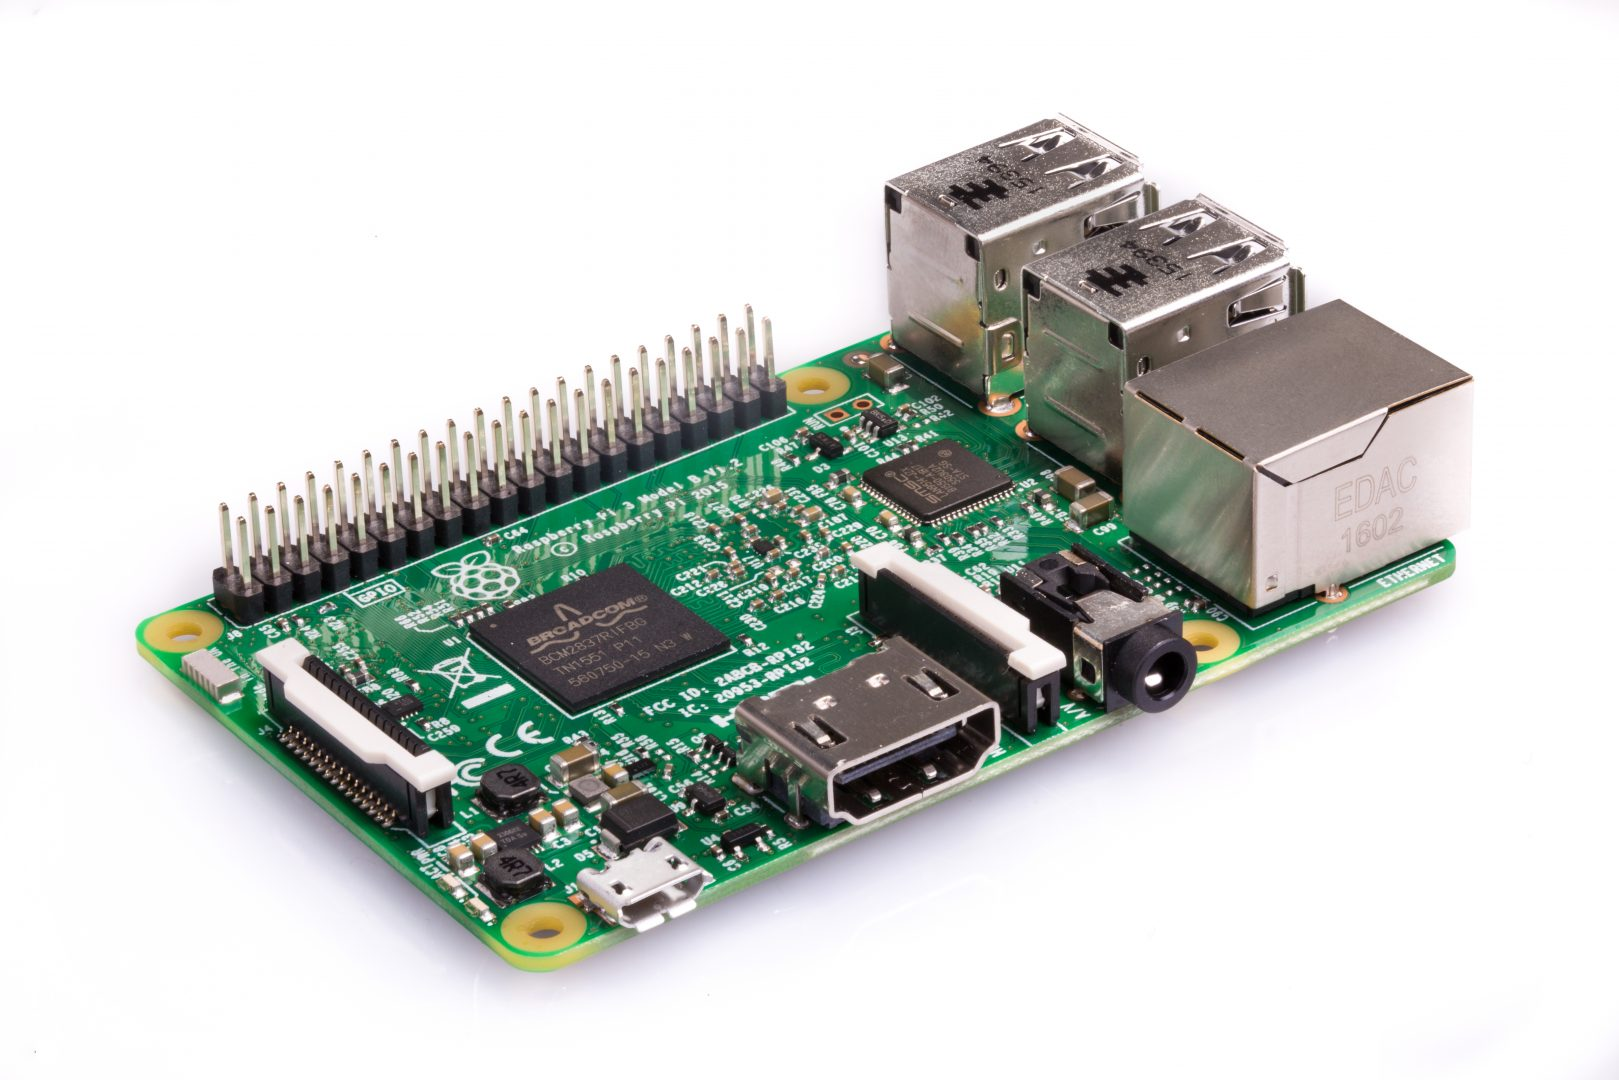
\includegraphics[width=0.6\textwidth]{raspberry.jpg}
		\caption{Exemplar da Raspberry Pi 3 modelo B.}
		\label{fig:raspberry}
	\end{center}
\end{figure}

\subsection{Câmara com lente olho de peixe}

A lente olho de peixe é uma lente grande-angular, uma vez que alcança ângulos de visão extremamente amplos. Além disso, produz uma forte distorção visual destinada a criar uma imagem panorâmica ou hemisférica ampla.  Em vez de produzir imagens com linhas retas de perspetiva, as lentes olho de peixe usam um mapeamento especial (por exemplo: ângulo equisólido), que dá às imagens uma aparência convexa não retilínea.

\subsubsection{Tipos de lentes}

Existem 2 tipos de lentes olho de peixe : circular e \textit{full-frame}. 

Os primeiros tipos de lentes olho de peixe desenvolvidos foram circulares, lentes que tomaram um hemisfério de 180º projetando um círculo no plano de imagem. Estas, têm 180º de ângulo de visão vertical, horizontal e diagonal. 

As lentes olho de peixe \textit{full-frame} ampliam o círculo da imagem para cobrir toda a estrutura retangular, designado por "olho de peixe de moldura completa". Desta forma, as lentes têm um ângulo de visão diagonal de 180º enquanto os ângulos vertical e horizontal de visão são menores. 

A figura ~\ref{fig:circularfullframe} representa as diferenças de plano de imagens obtidos com lente olho de peixe circular e olho de peixe \textit{full-frame}. Além disso também representa a diferenças em distâncias focais das lentes, na qual afeta o tamanho das imagens na plano de imagem.


A lente é aplicada num ambiente agrícola. Ao se utilizar a lente olho de peixe circular, esta mostra-nos um maior plano de imagem, contudo contém informação desnecessária, como o céu. Assim, torna-se mais vantajoso o uso da lente olho de peixe \textit{full-frame}, uma vez que fornece mais informação central e horizontal do campo de visão.

\begin{figure}[h!] %colocar figura a seguir ao texto anterior
	\begin{center}
		\leavevmode		
		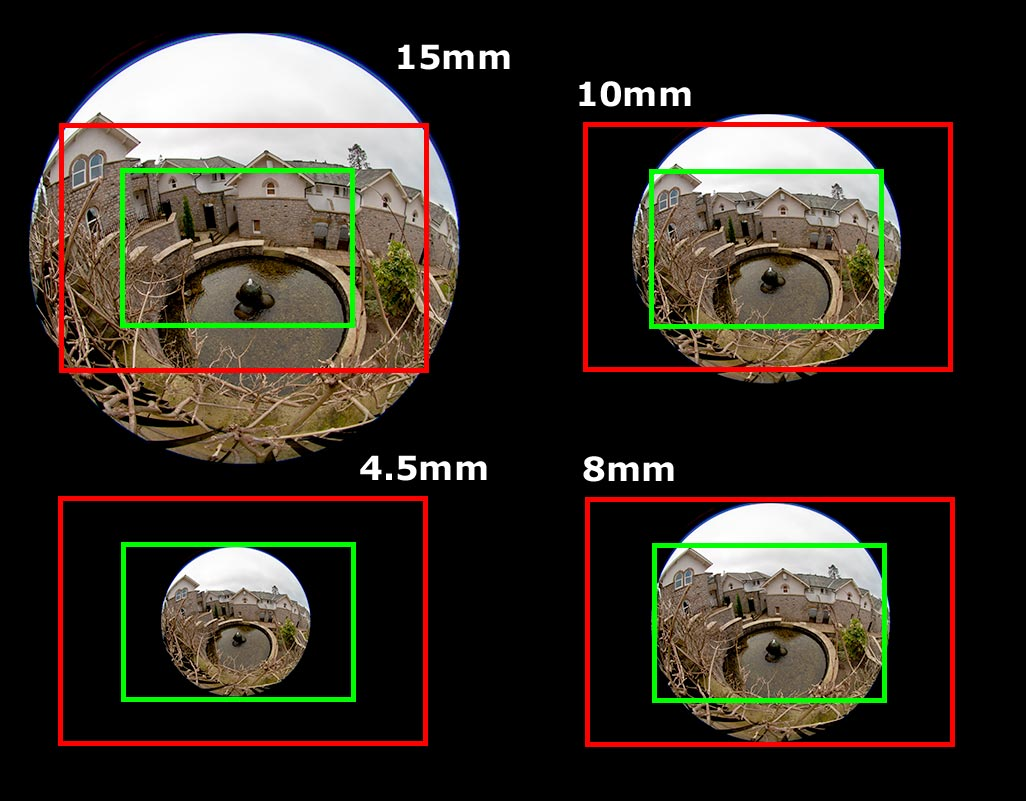
\includegraphics[width=0.6\textwidth]{circularfullframe.jpg}
		\caption{Diferença de ângulos de visão de lentes olho de peixe.}
		\label{fig:circularfullframe}
	\end{center}
\end{figure}


A lente especificamente escolhida é a representada na figura ~\ref{fig:lentfisheye}, com as seguintes especificações: 5 megapixel , ângulo de abertura de 160 graus (câmaras têm tipicamente 72 graus), resolução 1080p e com suporte para LED infravermelho para visão noturna.

\begin{figure}[h!]%colocar figura a seguir ao texto anterior
	\begin{center}
		\leavevmode		
		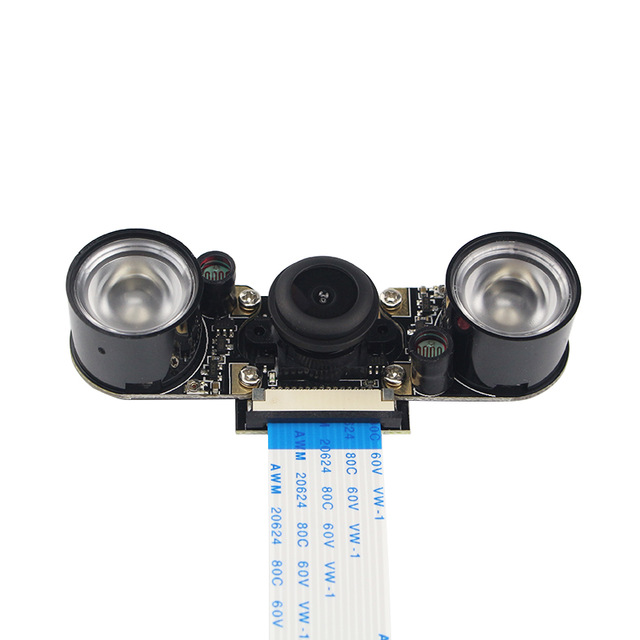
\includegraphics[width=0.4\textwidth]{lentfisheye}
		\caption{Câmara com lente olho de peixe e suporte para visão noturna.}
		\label{fig:lentfisheye}
	\end{center}
\end{figure}
